%************************************************
\chapter{Experiment 1A: UV-Visible Spectroscopy}
%************************************************
\begin{flushright}
August 16, 2012
\end{flushright}

\section{Objective}
	To
	\begin{enumerate}
		\item prepare 10, 25, 50 and 75 ppm solutions of Benzoic Acid in water
		\item use one of these for obtaining a spectrogram
		\item use three of these for calibration and find the concentration of the third experimentally
	\end{enumerate}

\section{Theory}
	This section is the same as and has been covered in the previous experiment.\\
	A few simple relations must be stated however, for clarity. Transmissivity or Transmission $(T)$ is related to observables by \autoref{1A_beer_lambert_t}, where $I$ is intensity of the light transmitted, $I_{0}$ is intensity of incident light, $\epsilon$ is extinction coefficient, $l$ is the path length and $c$ is concentration of the solution.\\
	Relation between Absorbance $(A)$ and intensity of light is as given by \autoref{1A_absorbance}. Clearly, $A$ has a linear relation with $\epsilon$ as given by \autoref{1A_beer_lambert} and we'll use this very relation to find the concentration of the `unknown' sample.
	
	\begin{equation}
		T=\frac{I}{I_{0}}=10^{-\epsilon l c}
		\label{1A_beer_lambert_t}
	\end{equation}
	\begin{equation}
		A=-\log{10}(\frac{I}{I_{0}})
		\label{1A_absorbance}
	\end{equation}
	\begin{equation}
		A=\epsilon l c
		\label{1A_beer_lambert}
	\end{equation}
	

\section{Procedure}
	\begin{enumerate}
		\item First calculated the mass of Benzoic Acid required for making a $25 mL$ a 250 ppm solution in water, to be \emph{6.25 mg}. \marginpar{\Maggie Just in case, $1 ppm = 1 uL / mL$}
		\item Weighed roughly the calculated amount of Benzoic Acid and transferred it to a volumetric flask of $25 mL$, and made the volume $25 mL$. This solution is henceforth referred to as the stock solution.\marginpar{\Lisa Used the upper meniscus \emph{consistently} for volume measurements \Bart But does that mean it wouldn't affect the result?}
		\item Calculated the volume of the stock solution required to prepare 10, 25, 50 and 75 ppm, 5 mL Benzoic Acid solutions.
		\item Using a graduated pipette, measured the precise volume in accordance with the calculations and transferred it to a $5 mL$ volumetric flask, and filled it to $5 mL$ of water. Repeated this step for all four concentrations and labelled the flasks accordingly.
		\item Calibrated the spectroscope with water first to suppress noise, if any.
		\item Used one of the concentrations to generate a spectrogram.
		\item Identified the maximum wavelength for use in Beer-Lambert law.
		\item Used three of the concentrations to calibrate and fourth as an unknown, using the spectroscope.
		\item Printed the spectrogram and noted the observations off of the screen for the known and unknown concentrations.
	\end{enumerate}

\section{Calculations and Measurements}
	Refer to \autoref{1A_stock} for the stock solution and to \autoref{1A_vary} for the variants.

	\begin{table}
		\myfloatalign
		\begin{tabularx}{\textwidth}{Xlll}
			\hline%
			Mass of salt 						& 	$0.0066$	& 	g\\
			Mass of paper 						& 	$0.0001$	& 	g\\
			Mass of Benzoic Acid				& 	$6.5$		&	mg\\
			Concentration of Benzoid Acid Used 	& 	$\frac{6500}{25}=260$ & ppm\\
			\hline%
		\end{tabularx}
		\caption{For the Stock Solution of Benzoic Acid}
		\label{1A_stock}
	\end{table}

	\begin{table}
		\myfloatalign
		\begin{tabularx}{\textwidth}{Xlll}
			\hline%
			10 ppm 	&	$\frac{50}{260}=0.192$	&	mL\\
			25 ppm 	&	$\frac{125}{260}=0.480$	&	mL\\
			10 ppm 	&	$\frac{250}{260}=0.961$	&	mL\\
			10 ppm 	&	$\frac{50}{375}=1.442$	&	mL\\ \hline%
		\end{tabularx}\\
		\caption{For varying concentrations of Benzoic Acid Solution}
		\label{1A_vary}
	\end{table}

\section{Spectroscopic Observations and Analysis}
	The maximum wavelength $(\lambda_{\text max})$ was found to be $524.00 nm$. Refer to \autoref{1A_lambdamax}. The Absorbance ($A$) for various concentration is given in \autoref{1A_conc_absorb}
	\begin{table}
		\myfloatalign
		\begin{tabularx}{\textwidth}{Xll}
			\hline
			\tableheadline{Wavelength $(\lambda)$} 	&	\tableheadline{Absorbance}\\
			$544.00 nm$								&	1.710\\
			$524.00 nm$								&	1.915\\		
			\hline
		\end{tabularx}
		\caption{Wavelengths Absorbed}
		\label{1A_lambdamax}
	\end{table}

	\begin{table}
		\myfloatalign
		\begin{tabularx}{\textwidth}{Xll}
			\hline
			\tableheadline{Concentration $(c)$} 	&	\tableheadline{Absorbance}\\
			$75 ppm$								&	1.902\\
			$50 ppm$								&	0.971\\
			$10 ppm$								&	0.237\\
			\hline
		\end{tabularx}
		\caption{Absorption for various Concentrations}
		\label{1A_conc_absorb}
	\end{table}
	Absorbance of `unknown' sample (25 ppm): 0.489
	\par
	In accordance with the application, the best fit for the three points was not linear and the concentration of the unknown sample was calculated to be 30.0720 ppm which amounts to a 20\% error.\\
	In accordance with least square straight line fit, we get the slope as 0.0249395 $\pm$ 20.34 \% but the intercept as -0.0856124 $\pm$ 310.2\%. In accordance with these numbers, the concentration works out to be 16.174 ppm, which is 35\% off. Refer to \autoref{1A_graph} for details.

	\begin{figure}[bth]
		\begin{center}
			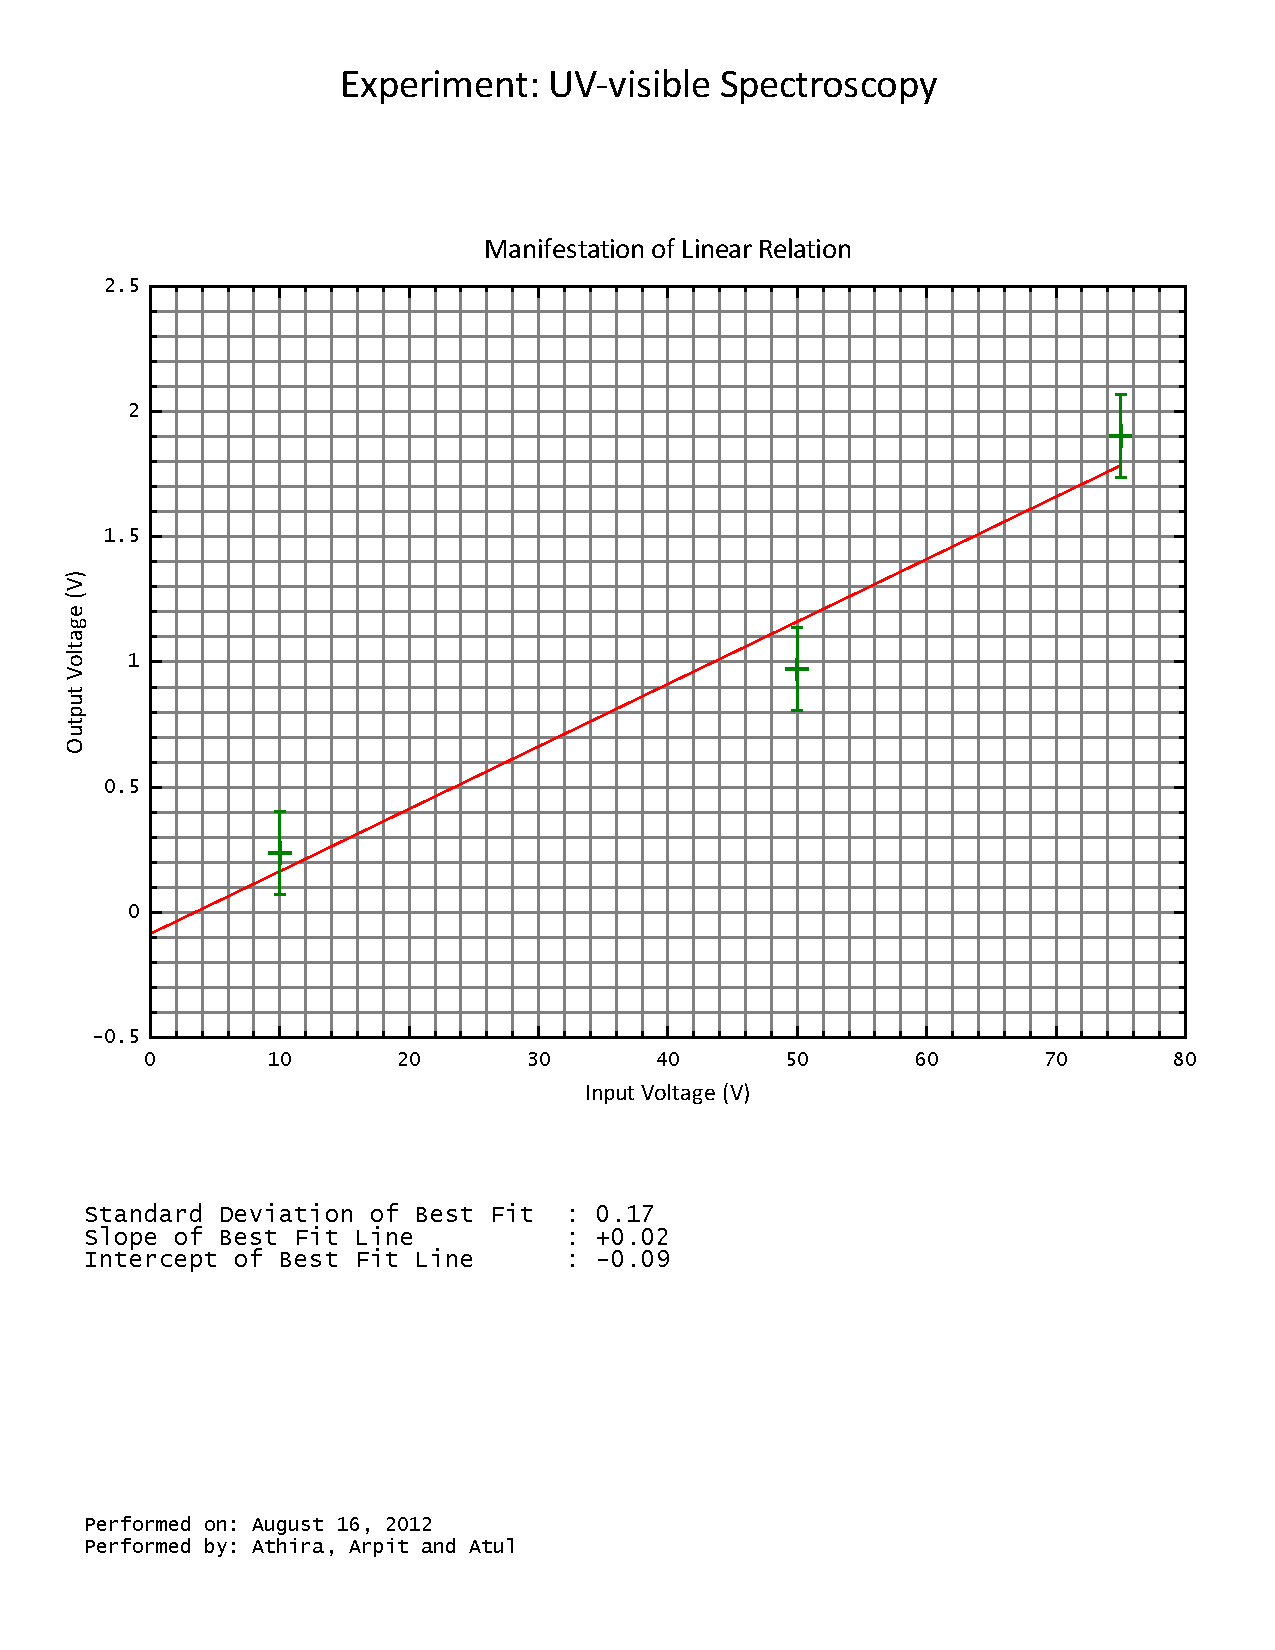
\includegraphics[width=1.3\linewidth]{gfx/1A_bestfit.pdf}
		\end{center}
	\caption[Least Square Fit]{Least Square Fit}
	\label{1A_graph}
	\end{figure}

\section{Acknowledgements}
I thank Ms. Sumyra, the PhD student, who helped us with the use of the spectroscope. I also acknowledge the contribution of Ms. Athira J. Nair and Mr. Arpit Porwal for the performance of the experiment as team members.